% !TEX root = morphkasten.tex

\section{Greifer}


%##############
\subsection{Greifer rund}

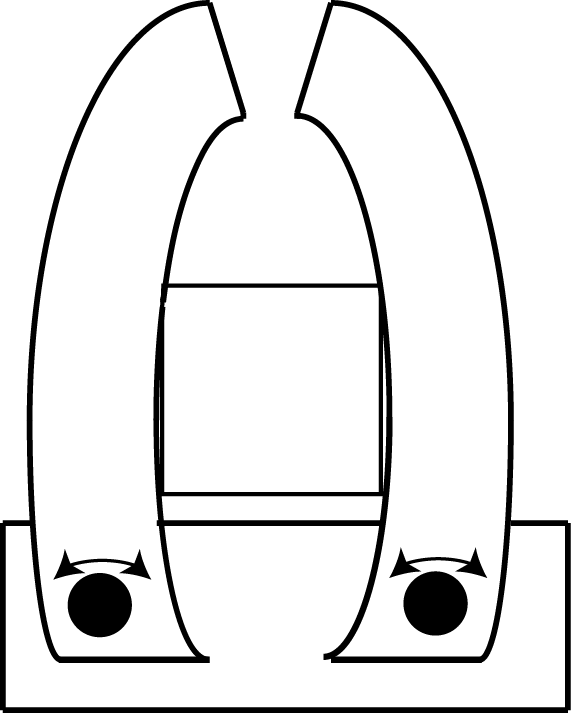
\includegraphics[width=0.5\textwidth]{fig/Greifer_rund.png}

\begin{table}[h]
\begin{tabular}{p{0.5\textwidth} | p{0.5\textwidth}}


 \textbf{Vorteile} & \textbf{Nachteile} \\ \hline
	 
\begin{itemize}
\item 2 Auflagepunkte am Container
\item Mit Zahnradübersetzung ist das Schliessen/Öffnen mit einem Motor möglich
\item keine Sensoren nötig um Schliessvorgang zu bestätigen
\item Automatische Zentrierung
\end{itemize}

 
 &
 
\begin{itemize}
\item Auf beiden Seiten hohe bzw. 2 Greiferbacken nötig um Stabilität zu garantieren
\item wenig Platz um Motor zu befestigen
\end{itemize}

\end{tabular}
\end{table}

\begin{table}[h]
\begin{tabular}{p{0.5\textwidth}p{0.5\textwidth}}


 \textbf{Risiken} & \\ \hline
	 
\begin{itemize}
\item Breitenbegrenzung überschreiten wegen der Länge des Greifers
\end{itemize}

 
\end{tabular}
\end{table}

\pagebreak


%##############
\subsection{Greifer gerade}

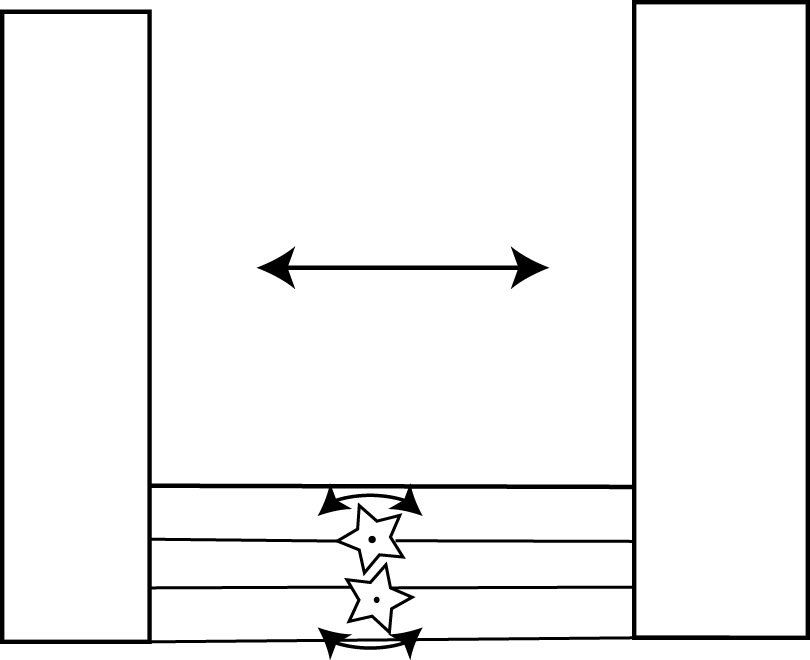
\includegraphics[width=0.5\textwidth]{fig/Greifer_gerade.png}

\begin{table}[h]
\begin{tabular}{p{0.5\textwidth} | p{0.5\textwidth}}


 \textbf{Vorteile} & \textbf{Nachteile} \\ \hline
	 
\begin{itemize}
\item grosse Auflagefläche für Container
\item Mit Zahnradübersetzung nur ein Motor zum Schliessen/Öffnen nötig
\end{itemize}

 
 &
 
\begin{itemize}
\item sehr breiter Greifer bei unpräziser Positionierung nötig
\item aufwändige Führung
\item hohes Gewicht
\item wenig Platz für Motor
\end{itemize}

\end{tabular}
\end{table}

\begin{table}[h]
\begin{tabular}{p{0.5\textwidth}p{0.5\textwidth}}


 \textbf{Risiken} & \\ \hline
	 
\begin{itemize}
\item Stabilität des Greifer fraglich
\item Motorenüberlastung
\end{itemize}

 
\end{tabular}
\end{table}

\pagebreak